%% using aastex version 6.2
\documentclass[twocolumn, dvipdfmx]{aastex62}
\usepackage{CJK}
\usepackage{textcomp}
\usepackage{graphicx}
\usepackage{here}
\usepackage{hhline}
\usepackage{longtable}

\def\red<#1>{\textcolor{red}{#1}}
\newcommand\aastex{AAS\TeX}
\newcommand\latex{La\TeX}

\received{\today}
\revised{\today}
\accepted{\today}
\submitjournal{ApJ}

\shortauthors{Goda \& Matsuo}

\begin{document}
\begin{CJK*}{UTF8}{min}

\title{Multiple populations of extrasolar gas giants}

\author{Shohei Goda}
\affil{\rm Department of Earth and Space Science, Graduate School of Science, Osaka University, 1-1, Machikaneyamacho, Toyonaka, Osaka 560-0043, Japan}

\author{Taro Matsuo}
\affiliation{\rm Department of Earth and Space Science, Graduate School of Science, Osaka University, 1-1, Machikaneyamacho, Toyonaka, Osaka 560-0043, Japan}


\begin{abstract}

There are two planetary formation scenarios: core accretion and gravitational disk instability. Most extrasolar gaseous objects discovered to date are thought to be formed from the core accretion, based on a fact that gaseous objects are preferentially observed around metal-rich host stars. Here, we present the 623 samples in 520 planetary systems comprising gaseous planets and brown dwarfs discovered by radial velocity measurements in three mass regimes with boundary values of 4 and 20 Jupiter-mass in terms of the host-star metallicity through performing a cluster analysis to the samples, minimizing an impact of the selection effect of radial velocity for the host star metallicity on the cluster analysis. The larger boundary is thought to be a boundary between planet and sub-stellar formations, being in agreement with the upper mass limit of the core-accreted planets predicted by some theoretical studies. The distributions of masses and eccentricities for the planetary samples with masses less than 20 Jupiter-mass orbiting the metal-rich stars can be naturally explained by the core accretion model. In contrast, the lower mass limit reflects a new population, planets with masses ranging from 4 to 20 Jupiter-mass orbiting the metal-poor stars, which are unlikely to be explained by the core-accretion model in terms of the distributions of planet mass and metallicity.


\end{abstract}

\vspace{1cm}

\keywords{methods: data analysis -- planets and satellites: terrestrial planets}


\section{Introduction} \label{sec:introduction}

Decades ago, the discussion of planetary formation in solar system was developed for the solar system \citep{1985prpl.conf.1100H}. Two representative formation scenarios for Jupiter have been proposed: Core accretion \citep{1974Icar...22..416P, 1980PThPh..64..544M, 1996Icar..124...62P} and disk instability \citep{1951PNAS...37....1K, 1997Sci...276.1836B, 2002Sci...298.1756M}. In theory, the two planetary-formation processes have different dependences on disk metallicity, which is defined as the ratio of the metal-number-density to hydrogen atoms, and planet mass \citep[e.g.,][]{2007ApJ...662.1282M}.

For the core accretion model, a proto-planet core easily grows to the critical core mass before the disk gas dissipates. This occurs because the disk metallicity reflects the building materials available for the core \citep{2004ApJ...616..567I, 2012A&A...541A..97M}. In fact, since the first planet orbiting a normal star was discovered \citep{1995Natur.378..355M}, large-sized radial velocity observations have revealed that, while the metallicities of stars hosting smaller planets such as Neptune-like planets and super-Earths are significantly lower than those of stars orbited by extrasolar gas giants \citep{2011arXiv1109.2497M, 2015AJ....149...14W}, the gas giants preferentially orbit metal-rich stars \citep[e.g.,][]{2003A&A...398..363S, 2005ApJ...622.1102F}. Because the central star and its surrounding protoplanetary disks are formed from a same molecular cloud, according to the primordial hypothesis, most gas giants are thought to have formed via the core accretion. Regarding the planet mass, the gas giants with planet mass up to 30 $\rm M_J$ are potentially formed via the core accretion \citep[e.g.,][]{2007ApJ...667..557T, 2016ApJ...823...48T}, where $\rm M_J$ represents Jupiter-mass. The number of the gas giants also decreases as the planet mass is higher \citep[e.g.,][]{2009A&A...501.1161M}.

For the disk instability scenario, there are various reports about the relationship between disk metallicity and disk-instability-induced planetary formation; there exists reports of negative correlation \citep{2006ApJ...636L.149C, 2007Arizona}, a very weak positive correlation \citep{2007ApJ...661L..77M}, and no correlation \citep{2002ApJ...567L.149B} in the metallicity range of the stars hosting the observed planets. Although the lower limit on the masses of the disk-instability-induced planets may exist \citep{2007ApJ...662.1282M}, the mass distribution of the gas giants formed via the disk instability still remains an open question. On the other hand, direct imaging of extrasolar planets orbiting HR8799, Formalhaut, and beta Pictoris reported in 2008 and 2010 \citep{2008Sci...322.1348M, 2008Sci...322.1345K, 2010Sci...329...57L}, respectively, confirmed the existing of outer planets, which can be naturally explained by the disk instability scenario rather than the extended core accretion with migration or planet-planet scattering \citep{2009ApJ...707...79D}. Thus, there may exist two populations originated from the two planetary formations.

Several previous studies showed that the gas giants are divided into two regimes with a boundary mass of 4 $\rm M_J$ and interpreted the two populations as an outcome originated from the two planetary formations \citep{2007A&A...464..779R, 2017A&A...603A..30S, 2018ApJ...853...37S}; while the gas giants lighter than 4 $\rm M_J$ are core-accreted planets, the gas giants more massive than 4 $\rm M_J$ may be formed through disk instability. However, it is possible to form very massive gas giants up to 30 $\rm M_J$ via the core accretion in theory \citep[e.g.,][]{2016ApJ...823...48T}(e.g., Tanigawa et al. 2008; Mordasini et al. 2009; Tanigawa \& Tanaka 2016) and the upper mass limit of the core-accreted planets is also expected to depend on the disk metallicity \citep{2012A&A...541A..97M}. Pebble accretion has been recently proposed as the third planetary formation scenario that enables massive core to be formed in the outer region beyond 10 AU \citep{2010A&A...520A..43O, 2012A&A...544A..32L}; more massive planets than the core-accreted planets are potentially formed thanks to wider hill radius. Thus, whether the boundary mass of 4 $\rm M_J$ can be applied as the upper boundaries of the bottom-up planetary formation scenarios such as the core accretion and pebble accretion is still unknown. Furthermore, although the previous studies did not consider the selection effects of the planet detections, the detection limits of the radial velocity measurements clearly depend on the metallicity of the host star (see Figure \ref{fig:bias}, (a)). 

In this paper, we re-investigate what the upper-mass limits of the bottom-up planetary formation scenarios are and explore the possibilities of multiple populations in the extrasolar planetary systems discovered to data through evaluating the distributions of the planet masses and eccentricities in the metal-rich and -poor regions, minimizing the measurement biases for the host-star metallicity and stellar mass, which are not derived by using the uniform method \citep[e.g.,][]{2004A&A...415.1153S, 2008A&A...487..373S}, and the detection biases of the radial velocity measurements. This paper is organized as follows. In Section \ref{sec:method}, we explain how the samples gathered for this study were composed and how the distributions of the planet masses, eccentricities, and semi-major axes in the metal-rich and -poor regions were evaluated. In Section \ref{sec:results}, we derive the boundary metallicity that is divided into two regions such that the distributions of the planet masses and semi-major axes are most different and investigate how the samples are divided with the Gaussian mixture model. In Section \ref{sec:discussion}, we discuss what the upper-mass limit of the gas giants formed via the bottom-up planetary formation is and whether the disk-instability-induced planetary formation occurs.


\section{Method} \label{sec:method}

In this section, we explain how to perform statistical analysis for extrasolar gaseous objects to understand their formation and evolution process and show how to deal with the selection effect of radial velocity measurements by which samples constructed for this study were detected. We also explain how we constructed the samples used in this study, determining the boundary between gas dwarfs such as Neptune-like planets and gaseous giants.


\subsection{Statistical Analysis} \label{subsec:analysis}

In this study, we first examined whether the distributions of semi-major axes and planet masses for gaseous objects arise from the selection effect of radial velocity measurements or from the dependency of the planetary formation and evolution process on the disk metallicity, constructing samples named as ``common-biased samples" that minimize an impact of the selection effect on the distributions, as to be discussed in Section \ref{subsec:common}. Given that the measurement errors follow a normal distribution, we sampled the host star metallicities and companion masses and divided the common-biased samples into two by a host-star metallicity. Using the ``anderson\_ksamp" module in Python, we compared the divided sub-samples in terms of planet mass and semi-major axis with two-sample Anderson-Darling test. Calculating the p-values derived from the two-sample Anderson-Darling test as a function of the host star metallicity, we searched for a boundary metallicity that divides the common-biased samples such that the distributions of companion masses and semi-major axes for the two sub-samples are most different. We iterated this procedure 1,000 times and finally evaluated how much different the two common-biased sub-samples are in terms of the semi-major axis and planet mass at the boundary metallicity. This result is shown in Section \ref{subsec:metal}.

Next, we explored how many populations exist in extrasolar gaseous objects discovered so far to investigate what the upper mass limit of the core-accreted planets is; we re-examined whether only two populations exist in the extrasolar gaseous objects, as shown in several previous studies \citep{2007A&A...464..779R, 2017A&A...603A..30S, 2018ApJ...853...37S}. Using the ``GaussianMixture" package in Python, we applied two-dimensional Gaussian mixture model to the diagram of host star metallicities versus companion masses and for the common-biased samples. The number of the Gaussian mixture models used for this cluster analysis ranges from 1 to 10. We determined the number of the components of the best Gaussian mixture model based on the Bayesian Information Criterion as well as to which each common-biased sample belong. Sampling the host star metallicities and companion masses, we repeated this procedure 1,000 times. This result is introduced in Section \ref{subsec:mass}.


\subsection{Common-biased Samples} \label{subsec:common}

In order to reveal the distributions of companion mass and orbital properties for companions orbiting various host-star metallicities, we gathered extrasolar gaseous objects discovered by radial velocity observations that precisely determine lower limit of companion mass, semi-major axis and eccentricity. The gathered objects are referred to as ``original samples" in this paper. Considering that there may exist the relation between the planetary-formation processes and the host-star metallicity, as discussed in Section \ref{sec:introduction}, it is preferable that the accuracies and terms of the radial velocity measurements, which detected the original samples, are independent of the host-star metallicity. This is because the original samples detected via radial velocity measurements are influenced by two selection effects: (i) limited sensitivity to long-period planets owing to short observation terms and (ii) limited sensitivity to low-mass planets owing to a lack of measurement precision in radial velocity measurement. The semi-major axis, $a|_{max}$ , and lower mass limit, $Mp\sin{i}|_{min}$, of the detectable companion can be determined by the accuracy, $\sigma$, and term, $\tau$, of the radial velocity measurements as below \citep{2008ApJ...677.1324T},
\begin{eqnarray}
\label{equ:a}
a|_{max} &=& M_{*}^{\frac{1}{3}}\tau^{\frac{2}{3}} , \\
\label{equ:Mp}
M_p\sin i|_{min} &\approx& 4.919\times10^{-3}P^{\frac{1}{3}}(1-e^2)^{\frac{1}{2}}M_{*}^{\frac{2}{3}}\sigma ,
\end{eqnarray}
where, $M_*$, $P$, and $e$ are the stellar mass, the orbital period and eccentricity of the companion, respectively. The region in which a companion can be detected is derived for each radial velocity measurement based on Equation (\ref{equ:a}) and (\ref{equ:Mp}). Figure \ref{fig:bias}, (a) compares the detectable probabilities of a companion with radial velocity measurements in a diagram of period versus lower limit of companion mass for the metal-rich and -poor regions. Note that the boundary metallicity was fixed to 0 dex. As shown in Figure \ref{fig:bias}, the accuracies of the radial velocity observations for the metal-poor original samples are clearly worse than those for the metal-rich ones. In contrast, the detectable semi-major axis for the original samples orbiting the metal-rich stars are slightly wider compared to those of the metal-poor samples. Thus, the selection effect of the radial velocity measurements depends on the host-star metallicity and affect the distributions of masses and semi-major axes for the two original sub-samples orbiting the metal-rich and -poor samples. 

Focusing on a fact that the distributions of masses and semi-major axes for the original samples discovered in the metal-rich (-poor) region are biased with the selection effect of the radial velocity measurements for the metal-rich (-poor) stars, we can minimize the impact of the different selection effects on the original samples through filtering the metal-rich (-poor) original samples with the selection effect in the metal-poor (-rich); the selection biases in the metal-rich and -poor stars were equalized (see Figure \ref{fig:bias}, (b)). In the filtering process, we judged whether each original sample simply satisfies the following criteria:
\begin{eqnarray}
M_p\sin{i}-M_p\sin{i}|_{min} &\geqq& \frac{1}{2}(a-a|_{max}) , \\
a &\leqq& a|_{max} .
\end{eqnarray}
The samples are included in the filtered samples only when the criteria are satisfied. Now, we refer the filtered samples to as ``common-biased samples."

\begin{figure}[t]
\begin{center}
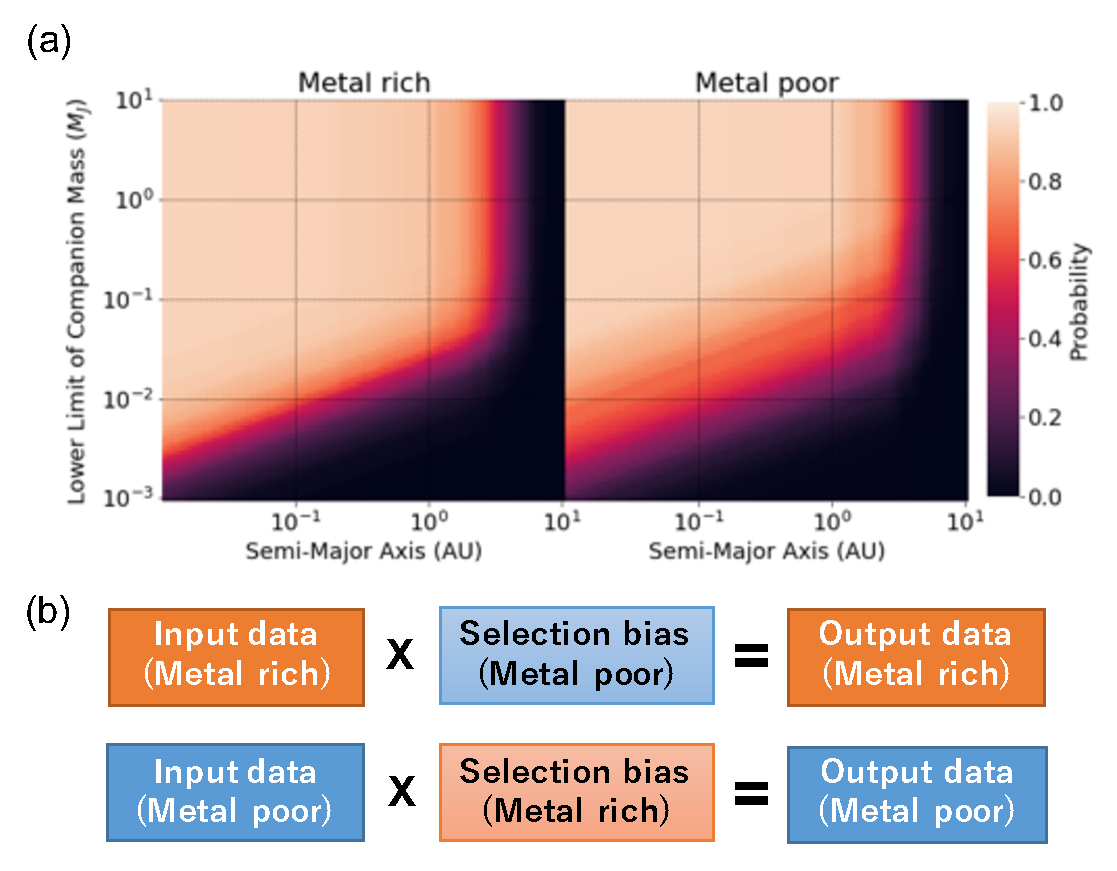
\includegraphics[width=9cm]{../../../Figure/selection_bias.pdf}
\caption{(a) Detection probabilities of a companion in a diagram of semi-major axis versus companion mass with the radial velocity measurements for the metal-rich (left) and -poor original samples (right) divided by a metallicity of 0 dex. The probability was defined as the fraction of the number of the radial velocity measurements that can detect a companion to the total of the measurements in each metallicity region. (b) Procedure for equalizing the selection biases included in the original samples in two different metallicity regions. The original metal-rich (-poor) samples were additionally filtered with the selection effects constructed from the radial velocity measurements of the metal-poor (-rich) samples. The filtered original samples were defined as ``common-biased samples" that are biased by a common selection effect. The filtering procedure judges whether the original samples can be detected by radial velocity measurements with the constructed selection effect, and the filtered samples are included in the common-biased samples only when the original samples are detectable. \label{fig:bias}}
\end{center}
\end{figure}


\subsection{Preparation of Samples} \label{subsec:preparation}

The original samples considered in this study are limited to companion objects detected by the radial velocity observations, allowing the orbital parameters to be characterized and lower limit of the companion mass to be determined. Essentially, the original samples are selected from those labeled ``Radial Velocity" in the ``detection method" column of the Extrasolar Planet Encyclopedia catalog as of the end of June 2018 \citep{2011A&A...532A..79S}. The radial velocities of the host stars orbited by the original samples, and the orbital periods and eccentricities of the original samples are also collected from the same catalog. The SWEET-Cat catalog was referred to for the metallicity and mass of the host star \citep{2013A&A...556A.150S, 2018A&A...620A..58S}; this catalog presents the uniformly derived stellar parameters of the planet host stars. For some of the original samples that are not listed in the SWEET-Cat catalog, the metallicities and masses measured by the Geneva-Copenhagen catalog \citep{2011A&A...530A.138C} the Padova database \citep{2000A&AS..141..371G}, and the BaSTI stellar model \citep{2018ApJ...856..125H} were applied and were calibrated by using regression lines determined from the correlations between the values in the SWEET-Cat catalog and those in the three catalogs to minimize measurement biases for host-star metallicities and masses. Using the stellar mass and the lower limit of companion mass was newly calculated based on Equation \ref{equ:Mp} because the host-star masses were revised.

The measurement accuracy and observation term for the radial velocity measurement of each original sample as the indicators of the selection effect were extracted from the exoplanets.org catalog. According to the Kepler’s third law shown in Equation \ref{equ:a}, the observation term and stellar mass provide the upper limit on the semi-major axis of a detectable companion with the radial velocity measurement of each original sample. Using the derived maximum semi-major axis, host-star mass and measurement accuracy, the lower limit on the mass of the detectable companion was derived based on Equation \ref{equ:Mp}.


\subsection{Boundary between Gas Giants and Neptune-like Planets} \label{subsec:boundary}

The gaseous objects were extracted from all the samples in the Extrasolar Planet Encyclopedia catalog in order to remove the impact of low-mass samples, such as Neptune-mass planets (gas dwarfs) and super-Earths, on this analysis. First, we determined the boundary mass between the gaseous and gas-dwarf objects from a perspective of both theory and observation. According to a previous study \citep{2004ApJ...604..388I}, gas-dwarf objects, which primarily consist of heavy-core objects such as Neptune and Uranus, have the potential to grow to the extent allowed by the core building materials inside their semi-major axes. This growth occurs via giant impacts in the inner region of the disk after the disk gas dissipates. However, this core growth is limited by the scattering effect of the heavy core increasing with greater distances from the central star. Therefore, the mass of a gas-dwarf object reaches a maximum at the semi-major axis, where the scattering effect begins to limit the core growth. Given that the ratio of collision-to-ejection probabilities for the heavy core is 0.1 and the core density is 1 $\rm g/cm^3$, the upper mass limit of the gas-dwarf object is approximately 0.1 $\rm M_J$ for dust surface densities of 3 times the Minimum Solar Nebulae Model value (MMSN).

From a standpoint of the observation, a boundary between gas giants and gas dwarfs at four times the Earth's radius has been observationally revealed by the Kepler data \citep{2012Natur.486..375B}. From the empirical planetary mass-radius relation \citep[e.g.,][]{2017A&A...604A..83B}:
\begin{equation}
\frac{R_p}{R_\oplus} \propto \left(\frac{M_p}{M_\oplus}\right)^{0.55\pm0.02} ,
\end{equation}
we found that the boundary of planetary mass is about 30 times the Earth's mass, corresponding to 0.1 $\rm M_J$. Thus, 0.1 $\rm M_J$ was applied in this study as the boundary mass between gas giants and gas dwarfs. The numbers of samples and their planetary systems considered in this study are 623 and 520, respectively.


\section{Results} \label{sec:results}

In this section, we quantitively show how different the distributions of the orbital properties and planet masses for the extrasolar gaseous objects orbiting the metal-rich and -poor regions are, minimizing the impact of the selection effect on their distributions. We also explore how many components exit in the extrasolar gaseous objects through classifying the common-biased samples with the Gaussian mixture model.


\subsection{Two Metallicity Regions} \label{subsec:metal}

We first determined the boundary of metallicity that divides the original samples into two such that the distributions of planet mass and semi-major axis in the two metal-rich and -poor regions are most different, respectively, using the method that considers the selection effects of the radial velocity measurements, as explained in Section \ref{subsec:analysis}. Figure \ref{fig:pvalue} shows the p-values derived by the two-sample Anderson-Darling test for the distributions of the semi-major axes and lower mass limits of the common-biased samples, changing the boundary of metallicity from -0.7 to 0.4 dex. Note that the common-biased samples, which were applied to the two-sample Anderson-Darling test, were constructed such that the impacts of the selection effects in the metal-rich and -poor regions on the common-biased sub-samples are equalized; the comparison between the two distributions of the common-biased sub-samples is not affected by the selection effects of the radial velocity measurements. We iterated the calculation 1,000 times and averaged the calculated p-values for each divided point to derive the mean and standard deviation of the p-values. The minimum p-values of the two-sample Anderson-Darling tests for the distributions of the semi-major axis and the planet mass were $2.4\times10^{-3}$ and $3.5\times10^{-5}/4.2\times10^{-5}$ at the metallicity of -0.04 and -0.29/-0.06 dex, respectively; thus, the planetary distributions in the metal-rich and -poor regions do not arise from the selection effect of the radial velocity measurements but from the planet formation and evolution. In this study, we used applied -0.05 dex as the boundary of metallicity through considering that the two minimum p-values are around -0.05 dex.

Next, we compared the distributions of the lower mass limit and semi-major axis for the common-biased sub-samples in the metal-rich and -poor regions that are divided by the boundary of metallicity. Figure \ref{fig:a_Mp} shows two scatter plots of the common-biased sub-samples in the metal-rich and -poor regions on the semi-major axis and lower-mass limit and compared the cumulative fractions of the common-biased sub-samples in terms of the semi-major axis and lower-mass limit, respectively. The gas giants with semi-major axis less than 0.1 AU and the planets more massive than about 5 $\rm M_J$ in the metal-poor region are relatively lack and excess compared to those in the metal-rich region, respectively. We discuss where the difference between the planetary distributions in the metal-rich and -poor regions comes from in Section \ref{sec:discussion}.

\begin{figure}[t]
\begin{center}
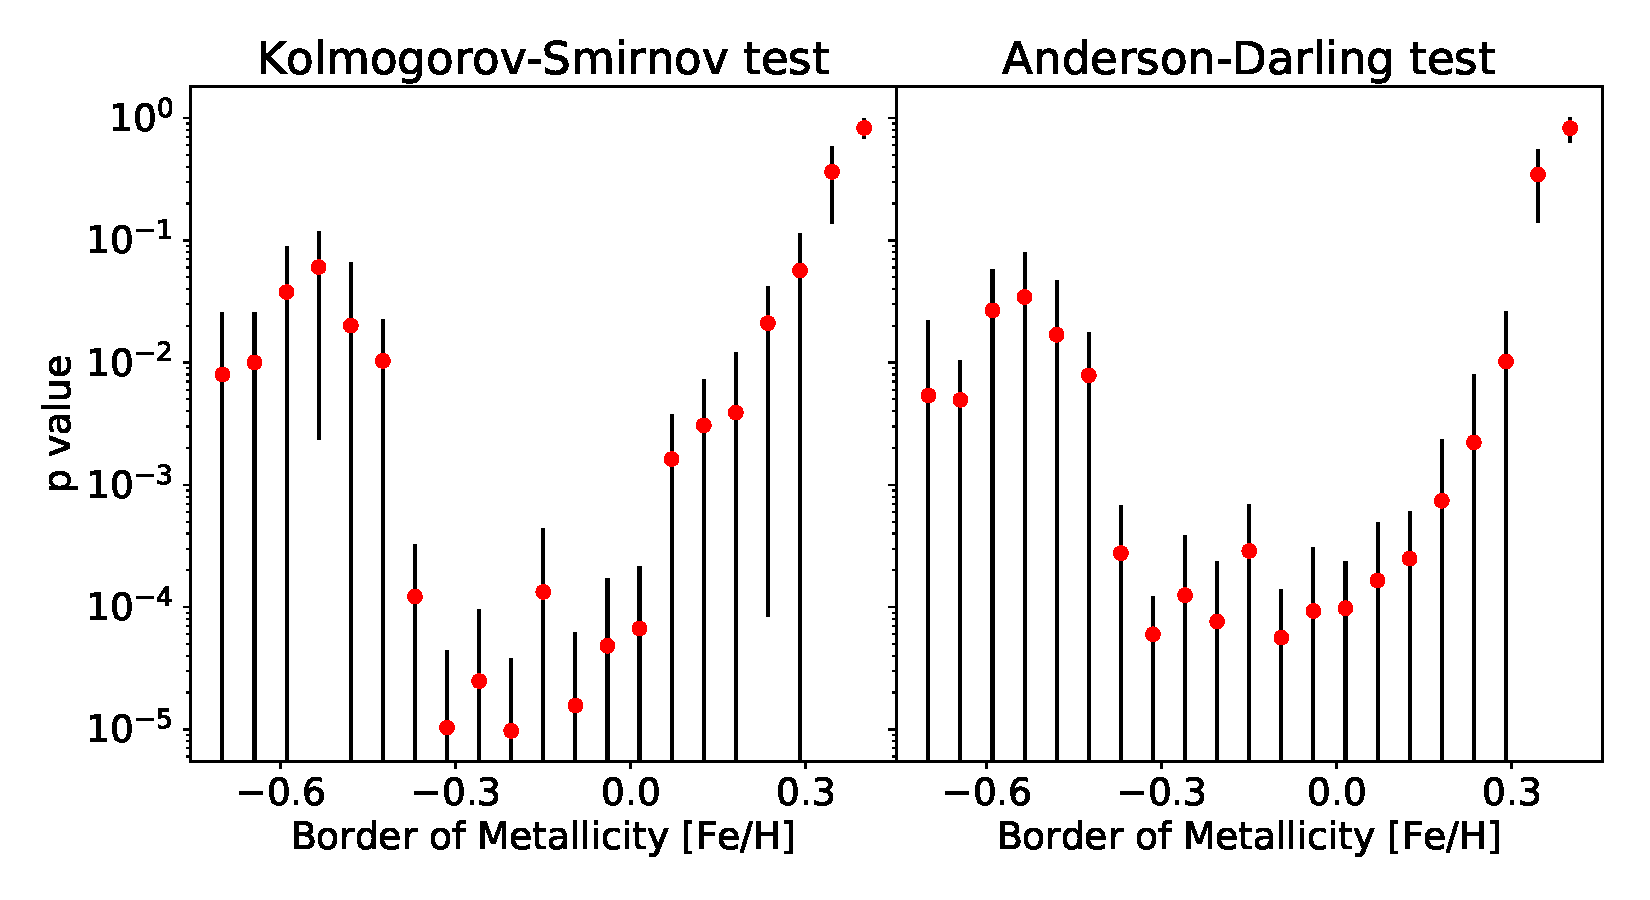
\includegraphics[width=9cm]{../../../Figure/pvalues_plot.pdf}
\caption{P-values calculated via two-sample Anderson-Darling tests for the semi-major axis (left) and the lower limit of the companion mass (right) of the original samples as a function of the boundary of metallicity. The red points and black vertical bars represent the mean p-values and their standard deviations, respectively. The number of the calculations for each boundary of metallicity is 1,000. \label{fig:pvalue}}
\end{center}
\end{figure}

\begin{figure}[t]
\begin{center}
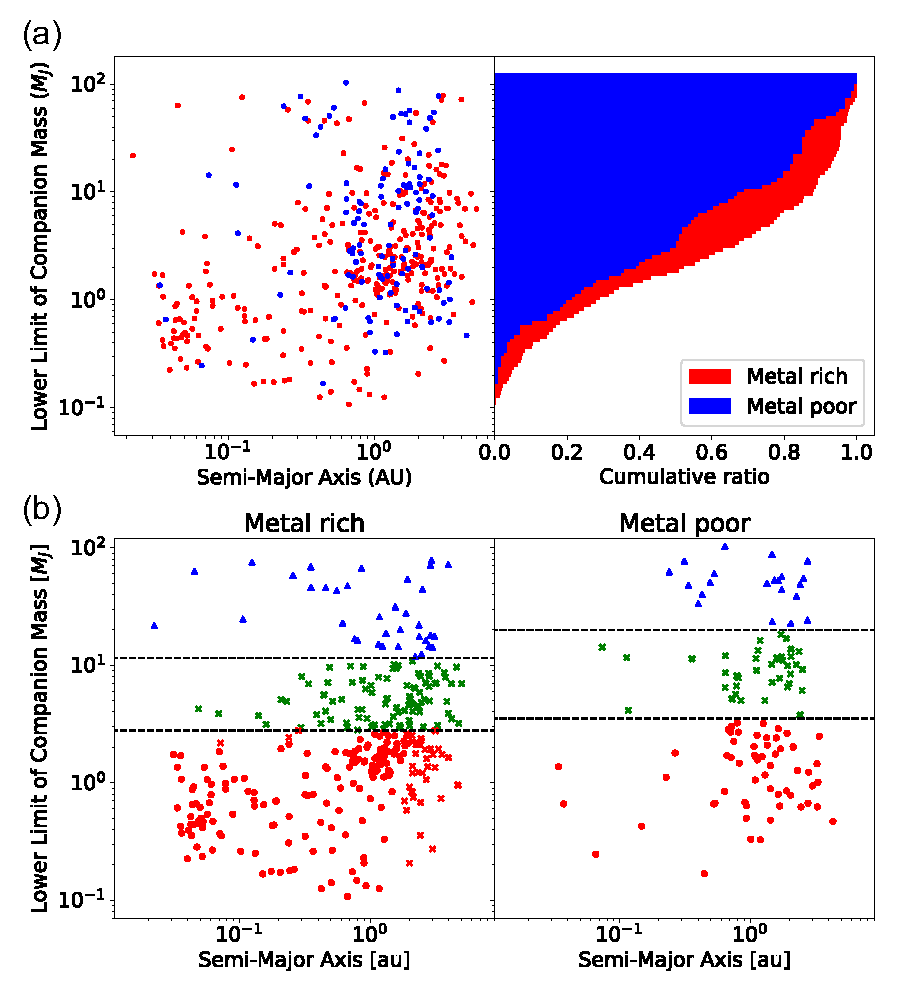
\includegraphics[width=9cm]{../../../Figure/a_Mp.pdf}
\caption{Distribution of the semi-major axes and lower limits of companion mass for the common-biased samples (upper left) and the cumulative distributions of semi-major axis (bottom) and lower limit of companion mass (right). The red and blue points/bins represent the metal-rich and -poor samples, respectively. An example among the 1,000 calculations was shown. \label{fig:a_Mp}}
\end{center}
\end{figure}


\subsection{Three Mass-Regimes of Gaseous Objects} \label{subsec:mass}

We classified the 623 common-biased samples into multiple sub-samples on the host-star metallicity and planet-mass plane with the Gaussian mixture model to explore how many sub-samples exist in the extrasolar gas giants discovered to data, given that each sub-sample follow a normal distribution \citep[e.g.,][]{2017A&A...603A..30S, 2018ApJ...853...37S}. Changing the number of the sub-samples, we evaluated each model with the Bayesian Information Criterion and found that the three-component model is suitable as the best Gaussian mixture model for the 623 common-biased samples. Figure \ref{fig:gmm} shows the best suited model for the common-biased samples. The common-biased samples are divided into three almost along two boundary masses of 4 and 20 $\rm M_J$. The three-component model results from relative paucity of the common-biased samples in two specific regions in the diagram of host-star metallicity versus companion mass; the two regions indicate gaseous objects with masses ranging from 20 to 30 $\rm M_J$ around both the metal-rich and -poor stars and those with masses ranging from 0.1 to 4 $\rm M_J$ around the metal-poor stars. The mean metallicity of the stars hosting the gaseous objects more with masses from 4 to 20 $\rm M_J$ is lower than that of the lighter samples and the mean metallicity of the samples more massive than 20 $\rm M_J$ is much lower than those of the other two sub-samples. Thus, the three-mass regimes exist in the extrasolar gaseous objects discovered so far instead of the two-mass regimes proposed by the previous studies \citep{2007A&A...464..779R, 2017A&A...603A..30S, 2018ApJ...853...37S}. Based on the theoretical studies on the maximum mass of the core-accreted planet \citep[e.g.,][]{2012A&A...541A..97M, 2016ApJ...823...48T}, we redefined the samples lighter than 20 $\rm M_J$ as planetary-mass objects and labeled the two sub-samples with masses from 0.1 to 4 $\rm M_J$ and from 4 to 20 $\rm M_J$ as ``intermediate-mass planets" and ``massive planets." In addition, the samples more massive than 20 $\rm M_J$ are labeled as ``brown dwarfs." Note that the boundary between planetary mass and brown dwarf objects established by the deuterium-burning minimum mass of ~ 10 $\rm M_J$ mentioned in a previous study is semantic \citep{2014prpl.conf..619C}; this boundary has no physical meaning from the perspective object evolution.

We next investigated the eccentricity distributions of the brown dwarfs, massive planets, and intermediate-mass planets in both the metal-rich and -poor regions, respectively. The upper panels of Figure \ref{fig:e_Mp} are scatter plots of the common-biased samples in the diagram of eccentricity versus companion mass in the metal-rich and -poor regions. The bottom panels are the cumulative fractions of the eccentricities for the three populations orbiting the metal-rich and -poor stars, respectively. The observational result common to the common-biased samples orbiting the metal-rich and -poor stars is that, while the eccentricities of the brown dwarfs uniformly distribute from 0 to 1, about 80 \% of the intermediate-mass planets have eccentricities smaller than 0.3. In contrast, the eccentricity distributions of the massive planets in the metal-rich and -poor regions are largely different; while the cumulative fraction of the eccentricities for the massive planets orbiting the metal-rich stars is close to that of the brown dwarf, that of the metal-poor massive planets is consistent with that of the intermediate-mass planets. In fact, as shown in Figure \ref{fig:e_ave}, the mean eccentricity of the massive planets decreases as the metallicity of the host star decreases. Thus, the eccentricity distributions also support the three-mass regimes of the extrasolar gaseous objects.

\begin{figure}[t]
\begin{center}
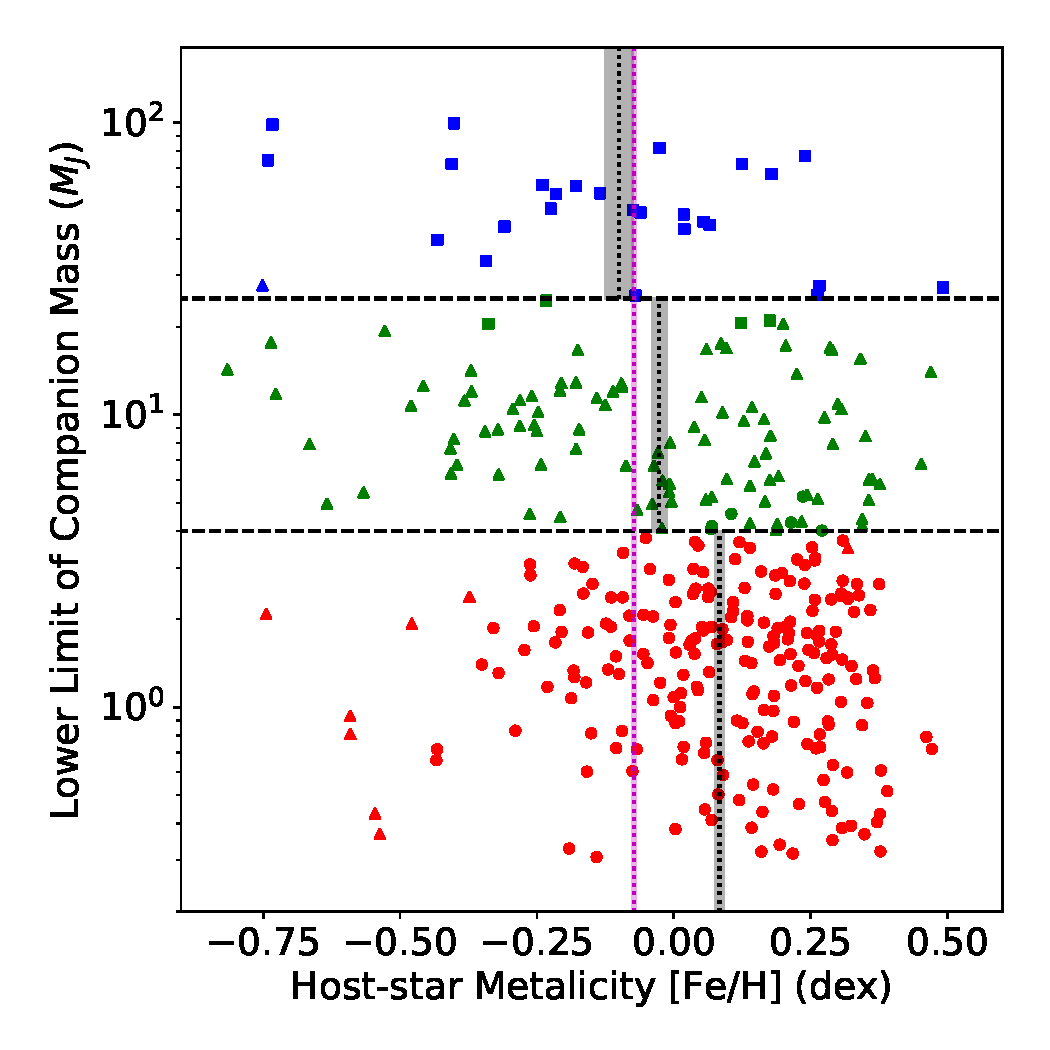
\includegraphics[width=7cm]{../../../Figure/gmm.pdf}
\caption{Distribution of the host-star metallicity and lower limit of companion masses for three common-biased sub-samples classified by the Gaussian mixture model. The different symbols of square, triangle, and circle represent the classified sub-samples. The blue, green, and red colors are three-mass regimes with two boundary masses of 4 and 20 $\rm M_J$ shown by the horizontal long-dashed lines. The vertical short dashed lines and gray regions in the three-mass regimes show the mean metallicity and its standard error in each regime, respectively. An example among the 1,000 calculations was shown. \label{fig:gmm}}
\end{center}
\end{figure}

\begin{figure}[t]
\begin{center}
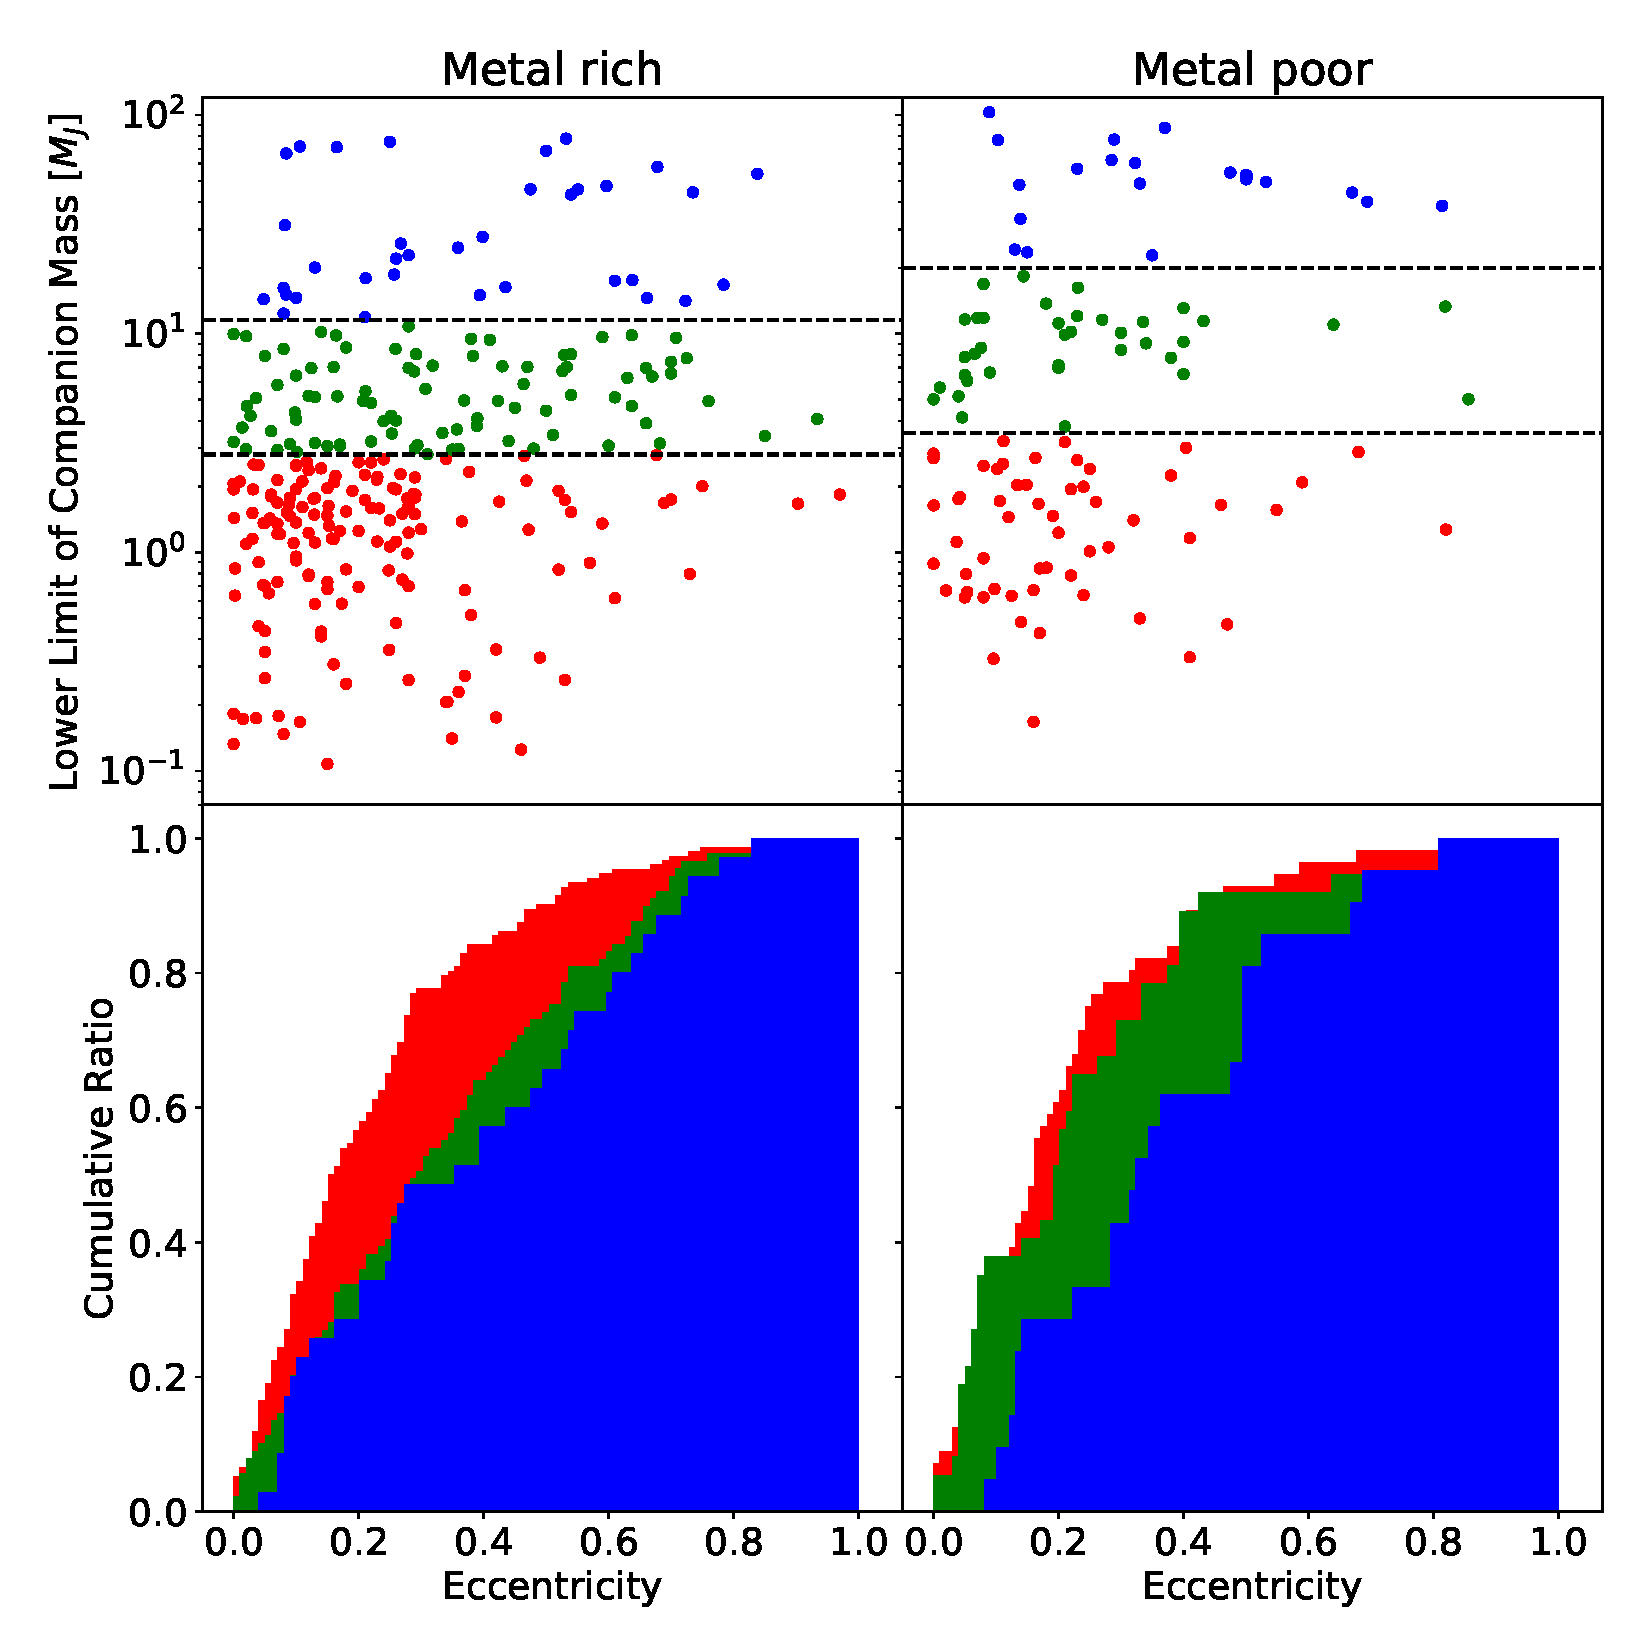
\includegraphics[width=9cm]{../../../Figure/e_Mp_merge.pdf}
\caption{Distributions of eccentricities and lower limits of companion mass (top) and the cumulative distributions of eccentricities for the common-biased samples orbiting the metal-rich and -poor regions (bottom). The horizontal lines and three colors represent same as those of Figure \ref{fig:gmm}. The white line is the cumulative uniform distribution. \label{fig:e_Mp}}
\end{center}
\end{figure}

\begin{figure}[t]
\begin{center}
\includegraphics[width=9cm]{../../../Figure/e_ave.pdf}
\caption{Histograms of eccentricities for the common-biased intermediate-mass planets (red) and massive ones (green) as a function of the host-star metallicity. The width of each bin was set to 0.26 dex. The height and vertical bar of each bin represent the mean eccentricity and its standard error for the common-biased intermediate-mass and massive planets belonging to each range. \label{fig:e_ave}}
\end{center}
\end{figure}


\section{Discussion} \label{sec:discussion}

In this section, we compare the above results of planetary mass and eccentricity distributions with previous studies and verify the relationship. We also discuss the behavior of planetary distributions in the metal-rich and -poor regions, comparing the observed dataset from the simulation of \cite{2012A&A...541A..97M}.


\subsection{Core Accretion Model} \label{subsec:accretion}

We compared the intermediate-mass and massive planets with the simulation data generated by \cite{2012A&A...541A..97M} that performed a population synthesis around 1 Solar mass within the framework of the core accretion model including planet growth and migration through planet-disk interaction. The upper panel of Figure \ref{fig:simulation} shows the distributions of semi-major axes and masses for the intermediate-mass and massive planets and the simulation samples in the metal-rich and -poor regions. The distribution of semi-major axes and masses for the intermediate-mass and massive planets are almost consistent with that for the simulation samples in the metal-rich region. In fact, as shown in the lower panel of Figure \ref{fig:simulation}, the mean masses for the observation and simulation samples have a good agreement in the metal-rich region. Note that the simulation samples were also filtered by both the selection biases of metal-rich and -poor regions and the observational samples were restricted to the intermediate-mass and massive planets orbiting host stars with masses ranging from 0.7 to 1.3 Solar mass.

On the other hand, an increase in the eccentricities of massive planets orbiting the metal-rich stars can be also explained by the following two models that are expanded from the core accretion model. One is planet-disk interaction at Lindblad and co-rotation resonances prior to gas dissipation \citep[e.g.,][]{2003ApJ...585.1024G}. According to the numerical simulations performed by \cite{2006A&A...447..369K}, the minimum planet mass for changing the disk gas into a high- eccentricity state is 3 $\rm M_J$ for the viscous coefficient of $10^{-5}$, which is almost consistent with the boundary between the intermediate-mass and massive planets. Another is dynamical instability induced by two closely separated gas giants and three gas giants, so called gravitational planet-planet interaction \citep[e.g.,][]{2013ApJ...775...42I}. The dynamical instability produces a gas giant with an eccentric orbit in outer region and a circular hot Jupiter in inner region through tidal circularization \citep[e.g.,][]{1996Sci...274..954R}. In fact, the paucity of the intermediate-mass planets that locate within 0.1 AU around metal-poor stars was confirmed; the gravitational planet-planet interaction occurs only around the metal-rich stars. The previous observations also confirmed that hot Jupiters orbit only the metal-rich stars \citep{2013ApJ...767L..24D, 2013A&A...560A..51A}.

Thus, the distributions of masses and eccentricities for intermediate-mass and massive planets orbiting the metal-rich stars can be naturally explained by the core accretion model; the upper mass limit of the core-accreted planets is thought to be around 20 $\rm M_J$, as to be discussed in Section \ref{subsec:scenarios}.

\begin{figure}[t]
\begin{center}
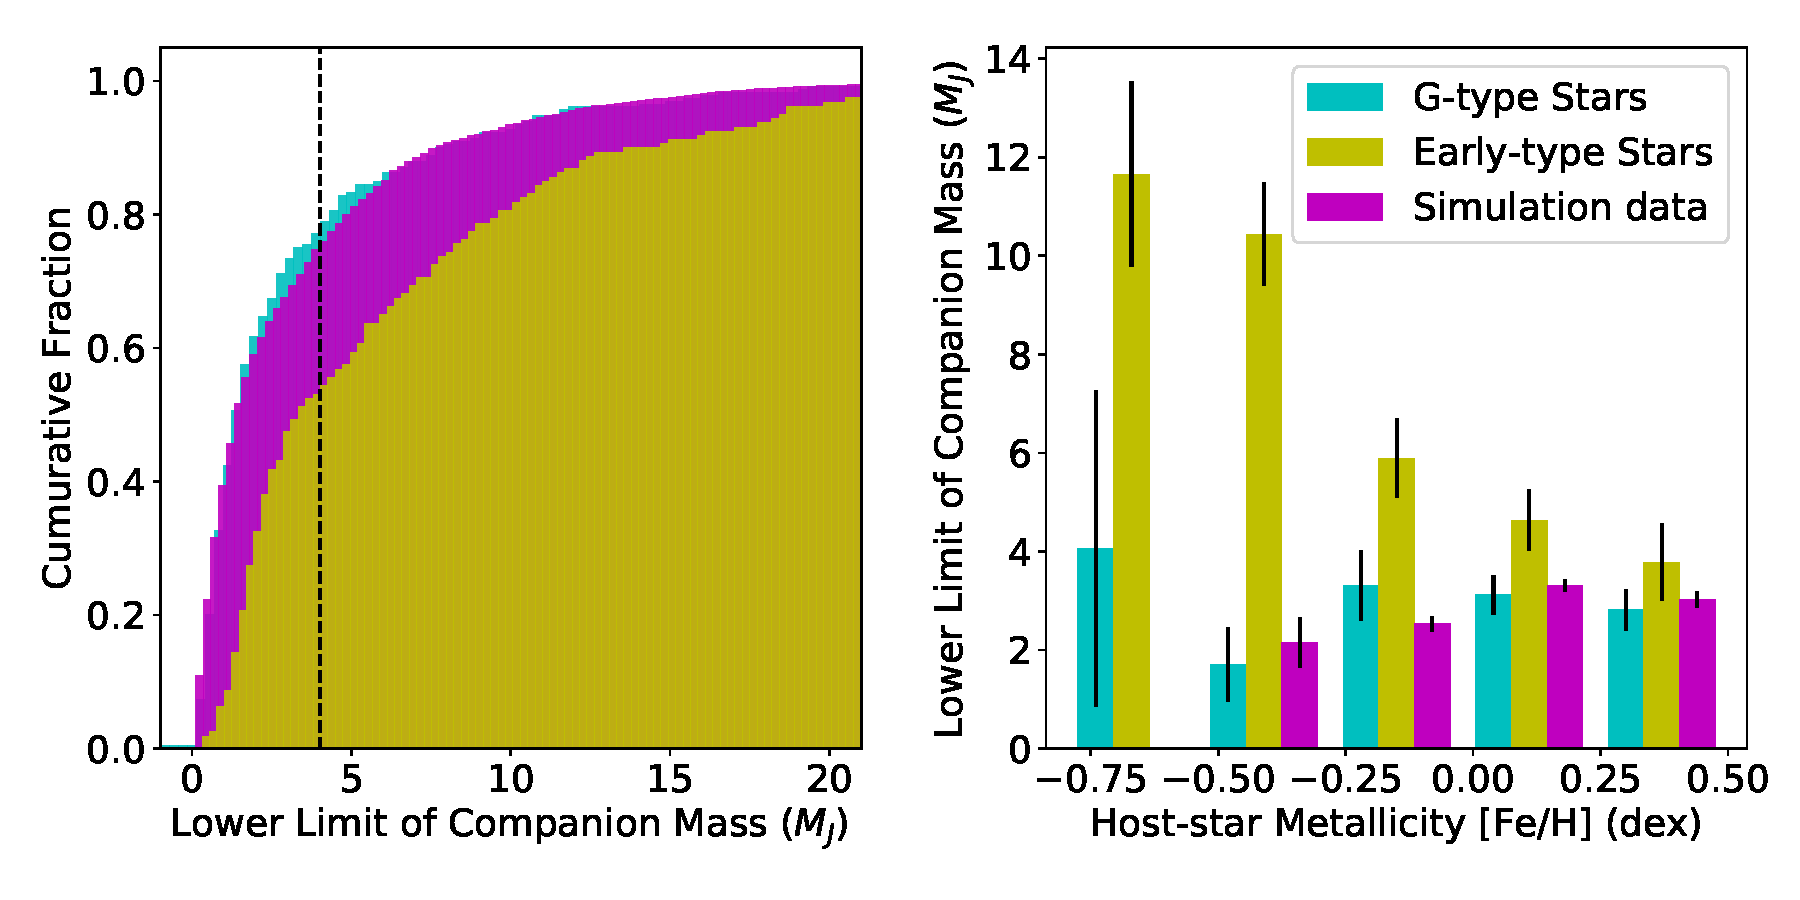
\includegraphics[width=9cm]{../../../Figure/simulation.pdf}
\caption{Distributions of semi-major axes and lower limit of companion masses for the common-biased intermediate-mass (red dots) and massive (green dots) planets and simulation samples with its corresponding mass (purple dots) generated by \cite{2012A&A...541A..97M} in the metal-rich (upper left) and -poor regions (upper right). Histograms of the mean masses for the common-biased intermediate-mass and massive planets (yellow bar) and simulation samples with its corresponding mass (purple bar) as a function of the host-star metallicity (lower panel). The error bar of each bar represents the standard error of the mean companion mass in each bin. \label{fig:simulation}}
\end{center}
\end{figure}


\subsection{Beyond the Core Accretion Model} \label{subsec:beyond}

In contrast, the distribution of semi-major axes and masses for the massive planets is not consistent with that for the simulation samples; there is an excess of the massive planets orbiting metal-poor stars and most of the planets locally distribute in the transition between 1 and 3 AU, in which the simulation samples are paucity. The excess of massive planets orbiting metal-poor stars differs from that expected form the core accretion formation theory in terms of the following two points. While more massive planets are likely to be formed around more metal-rich stars \citep{2012A&A...541A..97M}, the mean masses for the intermediate-mass and massive planets clearly increases as the metallicity decreases (Figure \ref{fig:simulation}). In addition, although a continuous decrease in the mass function of massive planets is theoretically predicted \citep{2009A&A...501.1161M}, the observation samples orbiting the metal-poor stars are clustered around 1 and 10 $\rm M_J$ (Figure \ref{fig:a_Mp}). The eccentricities of the massive planets orbiting metal-poor stars also differ from those around metal-rich stars (Figure \ref{fig:e_ave}); the eccentricities of the massive planets around the metal-poor stars do not seem to be enhanced through the planet-disk interaction prior to gas dissipation. Thus, the distributions of masses and eccentricities for the massive planets are unlikely to be explained by the bottom-up models.

An explanation for the excess massive planets orbiting metal-poor stars is that the disk instability acts in the vicinity of metal-poor stars, because a lower mass limit applies for planets formed via the disk instability mechanism (i.e., corresponding to an order of the Jeans mass \citep{2007ApJ...662.1282M, 2010Wiley}). As a result, a sharp increase appears in the planetary mass function around 4 $\rm M_J$. It is also accepted that planet formation due to disk instability tends to occur in the vicinity of metal-poor stars because the cooling timescale in the disk mid-plane is reduced owing to low disk opacity \citep{2006ApJ...636L.149C, 2007Arizona}. The low eccentricities of the massive planets orbiting the metal-poor stars are also consistent with the numerical simulations \citep{2004ApJ...609.1045M, 2010Wiley, 2011ApJ...731...74B} and the eccentricities of four gas giants orbiting HR8799 \citep{2017A&A...598A..83W}. Note that the four gas giants are located in a region beyond the core accretion model.


\subsection{Planetary Formation Scenarios} \label{subsec:scenarios}

Based on the above considerations, we compared the distribution of host star metallicities and companion masses for the 623 common-biased samples with the regions expected from the core accretion and disk instability models (Figure \ref{fig:metal_Mp}). The scarce regions appear in terms of companion mass, one at 0.1 to 4 $\rm M_J$ and one at 20 to 30 $\rm M_J$. Whereas the former arises from the rapid gas accretion onto the core, the latter represents a gap between binary star and planet formation. In other words, the two regions reflect the lower and upper mass limits of extrasolar gaseous objects that are formed by the planetary formation processes. In fact, the upper mass limit is almost consistent with the theoretical expectations \citep{2007ApJ...667..557T, 2012A&A...541A..97M, 2016ApJ...823...48T}.

While the intermediate-mass and massive planets orbiting the metal-rich stars can be explained by the core accretion model, the excess of massive planets is likely to be explained by the top-down model such as gravitational instability instead of the bottom-up scenario. The previous observational studies on dual planetary formation scenarios \citep{2007A&A...464..779R, 2017A&A...603A..30S, 2018ApJ...853...37S} showed that there exists a boundary mass of 4 to 10 $\rm M_J$ in the diagram of host star metallicities and masses for gaseous objects and mentioned that the boundary reflects the transition between the two planetary formations; the upper limit of the core-accreted planets is around 4 $\rm M_J$. However, we found that the boundary of 4 $\rm M_J$ reflects a population that is likely to be formed via disk instability and expected that planets with masses up to 20-30 $\rm M_J$ can be continuously formed by core-accretion around the metal-rich stars.

\begin{figure*}[t]
\begin{center}
\includegraphics[width=17cm]{../../../Figure/metal_Mp_size.pdf}
\caption{Distribution of host-star metallicities and companion masses for all 623 common-biased samples. Comparison of all 623 samples (black dots) with expectations from core accretion and disk instability theories in terms of host-star metallicity and planetary mass distributions. The red and green regions indicate the objects formed by core accretion and disk instability, respectively. The error bars indicate the 1-sigma measurement errors.
 \label{fig:metal_Mp}}
\end{center}
\end{figure*}

%\acknowledgments

\clearpage
%\vspace{5mm}


\begin{thebibliography}{}

\bibitem[Adibekyan et al.(2013)]{2013A&A...560A..51A} Adibekyan, V.~Z., Figueira, P., Santos, N.~C., et al.\ 2013, \aap, 560, A51
\bibitem[Bashi et al.(2017)]{2017A&A...604A..83B} Bashi, D., Helled, R., Zucker, S., \& Mordasini, C.\ 2017, \aap, 604, A83
\bibitem[Boss(1997)]{1997Sci...276.1836B} Boss, A.~P.\ 1997, Science, 276, 1836
\bibitem[Boss(2002)]{2002ApJ...567L.149B} Boss, A.~P.\ 2002, \apjl, 567, L149
\bibitem[Boss(2011)]{2011ApJ...731...74B} Boss, A.~P.\ 2011, \apj, 731, 74
\bibitem[Buchhave et al.(2012)]{2012Natur.486..375B} Buchhave, L.~A., Latham, D.~W., Johansen, A., et al.\ 2012, \nat, 486, 375
\bibitem[Cai et al.(2006)]{2006ApJ...636L.149C} Cai, K., Durisen, R.~H., Michael, S., et al.\ 2006, \apjl, 636, L149
\bibitem[Casagrande et al.(2011)]{2011A&A...530A.138C} Casagrande, L., Sch{\"o}nrich, R., Asplund, M., et al.\ 2011, \aap, 530, A138
\bibitem[Chabrier et al.(2014)]{2014prpl.conf..619C} Chabrier, G., Johansen, A., Janson, M., \& Rafikov, R.\ 2014, Protostars and Planets VI, 619
\bibitem[Chiang et al.(2002)]{2002ApJ...564L.105C} Chiang, E.~I., Fischer, D., \& Thommes, E.\ 2002, \apjl, 564, L105
\bibitem[Dawson \& Murray-Clay(2013)]{2013ApJ...767L..24D} Dawson, R.~I., \& Murray-Clay, R.~A.\ 2013, \apjl, 767, L24
\bibitem[Dodson-Robinson et al.(2009)]{2009ApJ...707...79D} Dodson-Robinson, S.~E., Veras, D., Ford, E.~B., \& Beichman, C.~A.\ 2009, \apj, 707, 79
\bibitem[Dupuy \& Liu(2011)]{2011ApJ...733..122D} Dupuy, T.~J., \& Liu, M.~C.\ 2011, \apj, 733, 122
\bibitem[Durisen et al.(2007)]{2007Arizona} Durisen, R. H., Reipurth, V. Jewitt, Keil, K., et al.\ 2007, Univ. of Arizona Press, Tucson 951, 607-622
\bibitem[Fischer \& Valenti(2005)]{2005ApJ...622.1102F} Fischer, D.~A., \& Valenti, J.\ 2005, \apj, 622, 1102
\bibitem[Girardi et al.(2000)]{2000A&AS..141..371G} Girardi, L., Bressan, A., Bertelli, G., \& Chiosi, C.\ 2000, \aaps, 141, 371
\bibitem[Goldreich \& Sari(2003)]{2003ApJ...585.1024G} Goldreich, P., \& Sari, R.\ 2003, \apj, 585, 1024
\bibitem[Hayashi et al.(1985)]{1985prpl.conf.1100H} Hayashi, C., Nakazawa, K., \& Nakagawa, Y.\ 1985, Protostars and Planets II, 1100
\bibitem[Hidalgo et al.(2018)]{2018ApJ...856..125H} Hidalgo, S.~L., Pietrinferni, A., Cassisi, S., et al.\ 2018, \apj, 856, 125
\bibitem[Ida \& Lin($2004a$)]{2004ApJ...604..388I} Ida, S., \& Lin, D.~N.~C.\ 2004a, \apj, 604, 388
\bibitem[Ida \& Lin($2004b$)]{2004ApJ...616..567I} Ida, S., \& Lin, D.~N.~C.\ 2004b, \apj, 616, 567
\bibitem[Ida et al.(2013)]{2013ApJ...775...42I} Ida, S., Lin, D.~N.~C., \& Nagasawa, M.\ 2013, \apj, 775, 42
\bibitem[Kalas et al.(2008)]{2008Sci...322.1345K} Kalas, P., Graham, J.~R., Chiang, E., et al.\ 2008, Science, 322, 1345
\bibitem[Kley \& Dirksen(2006)]{2006A&A...447..369K} Kley, W., \& Dirksen, G.\ 2006, \aap, 447, 369
\bibitem[Kuiper(1951)]{1951PNAS...37....1K} Kuiper, G.~P.\ 1951, Proceedings of the National Academy of Science, 37, 1
\bibitem[Lagrange et al.(2010)]{2010Sci...329...57L} Lagrange, A.-M., Bonnefoy, M., Chauvin, G., et al.\ 2010, Science, 329, 57
\bibitem[Lambrechts \& Johansen(2012)]{2012A&A...544A..32L} Lambrechts, M., \& Johansen, A.\ 2012, \aap, 544, A32
\bibitem[Lee et al.(2012)]{2012MNRAS.424.2832L} Lee, K.~J., Guillemot, L., Yue, Y.~L., Kramer, M., \& Champion, D.~J.\ 2012, \mnras, 424, 2832
\bibitem[Ma \& Ge(2014)]{2014MNRAS.439.2781M} Ma, B., \& Ge, J.\ 2014, \mnras, 439, 2781
\bibitem[Marois et al.(2008)]{2008Sci...322.1348M} Marois, C., Macintosh, B., Barman, T., et al.\ 2008, Science, 322, 1348
\bibitem[Matsuo et al.(2007)]{2007ApJ...662.1282M} Matsuo, T., Shibai, H., Ootsubo, T., \& Tamura, M.\ 2007, \apj, 662, 1282
\bibitem[Mayor \& Queloz(1995)]{1995Natur.378..355M} Mayor, M., \& Queloz, D.\ 1995, \nat, 378, 355
\bibitem[Mayer et al.(2002)]{2002Sci...298.1756M} Mayer, L., Quinn, T., Wadsley, J., \& Stadel, J.\ 2002, Science, 298, 1756
\bibitem[Mayer et al.(2004)]{2004ApJ...609.1045M} Mayer, L., Quinn, T., Wadsley, J., \& Stadel, J.\ 2004, \apj, 609, 1045
\bibitem[Mayer et al.(2007)]{2007ApJ...661L..77M} Mayer, L., Lufkin, G., Quinn, T., \& Wadsley, J.\ 2007, \apjl, 661, L77
\bibitem[Mayer(2010)]{2010Wiley} Mayer, L.\ 2010, Formation via Disk Instability. Formation and Evolution of Exoplanets, by Barns, R. (eds.) Wiley, 71-99
\bibitem[Mayor et al.(2011)]{2011arXiv1109.2497M} Mayor, M., Marmier, M., Lovis, C., et al.\ 2011, arXiv:1109.2497
\bibitem[Mizuno(1980)]{1980PThPh..64..544M} Mizuno, H.\ 1980, Progress of Theoretical Physics, 64, 544
\bibitem[Mordasini et al.(2009)]{2009A&A...501.1161M} Mordasini, C., Alibert, Y., Benz, W., \& Naef, D.\ 2009, \aap, 501, 1161
\bibitem[Mordasini et al.(2012)]{2012A&A...541A..97M} Mordasini, C., Alibert, Y., Benz, W., Klahr, H., \& Henning, T.\ 2012, \aap, 541, A97
\bibitem[Ormel \& Klahr(2010)]{2010A&A...520A..43O} Ormel, C.~W., \& Klahr, H.~H.\ 2010, \aap, 520, A43
\bibitem[Perri \& Cameron(1974)]{1974Icar...22..416P} Perri, F., \& Cameron, A.~G.~W.\ 1974, \icarus, 22, 416
\bibitem[Pollack et al.(1996)]{1996Icar..124...62P} Pollack, J.~B., Hubickyj, O., Bodenheimer, P., et al.\ 1996, \icarus, 124, 62
\bibitem[Rasio \& Ford(1996)]{1996Sci...274..954R} Rasio, F.~A., \& Ford, E.~B.\ 1996, Science, 274, 954
\bibitem[Ribas \& Miralda-Escud{\'e}(2007)]{2007A&A...464..779R} Ribas, I., \& Miralda-Escud{\'e}, J.\ 2007, \aap, 464, 779
\bibitem[Santos et al.(2003)]{2003A&A...398..363S} Santos, N.~C., Israelian, G., Mayor, M., Rebolo, R., \& Udry, S.\ 2003, \aap, 398, 363
\bibitem[Santos et al.(2004)]{2004A&A...415.1153S} Santos, N.~C., Israelian, G., \& Mayor, M.\ 2004, \aap, 415, 1153
\bibitem[Santos et al.(2013)]{2013A&A...556A.150S} Santos, N.~C., Sousa, S.~G., Mortier, A., et al.\ 2013, \aap, 556, A150
\bibitem[Santos et al.(2017)]{2017A&A...603A..30S} Santos, N.~C., Adibekyan, V., Figueira, P., et al.\ 2017, \aap, 603, A30
\bibitem[Schlaufman(2018)]{2018ApJ...853...37S} Schlaufman, K.~C.\ 2018, \apj, 853, 37
\bibitem[Schneider et al.(2011)]{2011A&A...532A..79S} Schneider, J., Dedieu, C., Le Sidaner, P., Savalle, R., \& Zolotukhin, I.\ 2011, \aap, 532, A79
\bibitem[Sousa et al.(2008)]{2008A&A...487..373S} Sousa, S.~G., Santos, N.~C., Mayor, M., et al.\ 2008, \aap, 487, 373
\bibitem[Sousa et al.(2018)]{2018A&A...620A..58S} Sousa, S.~G., Adibekyan, V., Delgado-Mena, E., et al.\ 2018, \aap, 620, A58
\bibitem[Tanigawa \& Ikoma(2007)]{2007ApJ...667..557T} Tanigawa, T., \& Ikoma, M.\ 2007, \apj, 667, 557
\bibitem[Tanigawa \& Tanaka(2016)]{2016ApJ...823...48T} Tanigawa, T., \& Tanaka, H.\ 2016, \apj, 823, 48
\bibitem[Torres et al.(2008)]{2008ApJ...677.1324T} Torres, G., Winn, J.~N., \& Holman, M.~J.\ 2008, \apj, 677, 1324
\bibitem[Wang \& Fischer(2015)]{2015AJ....149...14W} Wang, J., \& Fischer, D.~A.\ 2015, \aj, 149, 14
\bibitem[Wertz et al.(2017)]{2017A&A...598A..83W} Wertz, O., Absil, O., G{\'o}mez Gonz{\'a}lez, C.~A., et al.\ 2017, \aap, 598, A83

\end{thebibliography}

%\appendix

%\section{Unconsidered Factors}

%\begin{figure}[H]
%\begin{center}
%\includegraphics[width=12cm]{../../../Figure/bias_G_K.pdf}
%\caption{\label{fig:bias_G_K}}
%\end{center}
%\end{figure}


\end{CJK*}
\end{document}
